% include the figures path relative to the master file
%\graphicspath{ {./content/method/figures/} }

\section{Background}\label{sec:review}
This section reviews works straightly addressing the problem of classifying \gls{oct} volumes as normal or abnormal, regardless of the targeted pathology.
The methods are categorized in terms of their learning strategy, namely supervised or semi-supervised learning.

\begin{figure*}[t]
  \centering{
  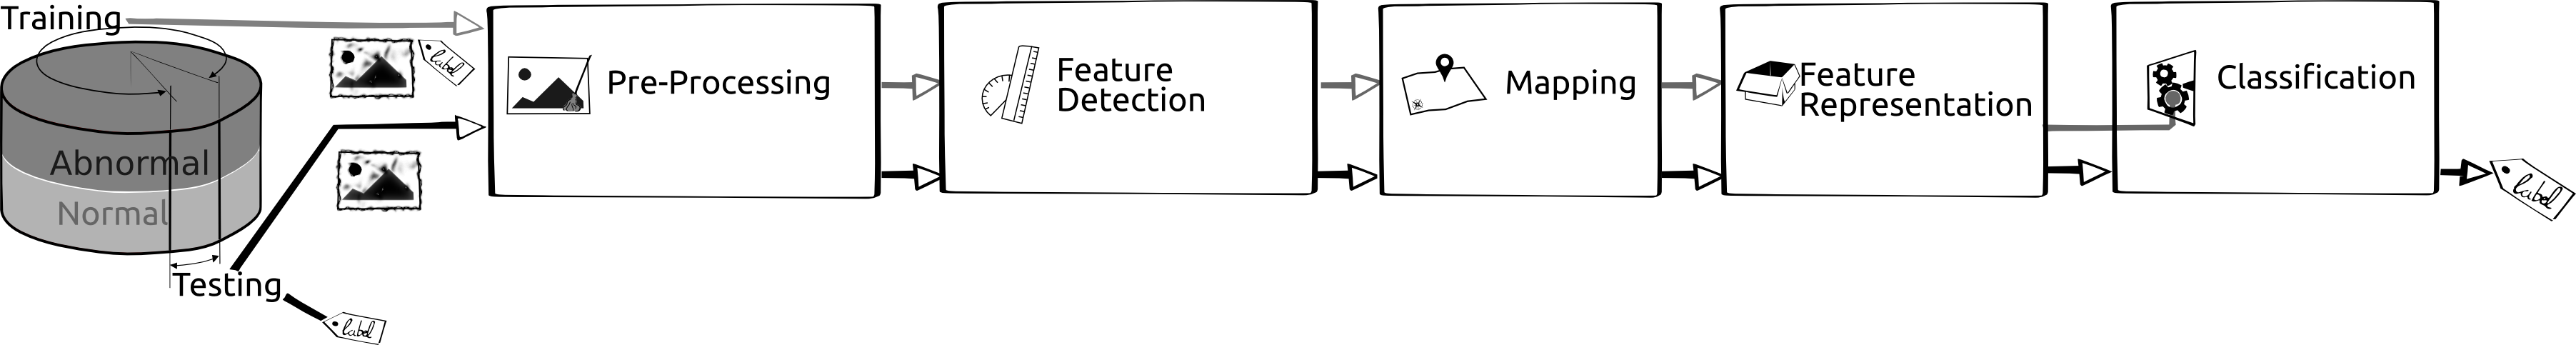
\includegraphics[width=1\linewidth]{./content/method/figures/ml-2}}
  \caption{Common framework}
  \label{fig:ML-scheme}
\end{figure*}

\subsection{Supervised methods}
% Common framework
% \added[id=mojh]{
%   All the previously mentioned methods follow a similar pipeline or framework, which consists of different steps.
%   We categorized these steps as pre-processing, feature extraction, mapping, feature representation and finally classification, as it is shown in Fig.\,\ref{fig:ML-scheme}.

%   Pre-processing of \gls{oct} volumes, as noted in Sect.~\ref{sec:review}, consists of denoising, flattening the retinal curvature, aligning the B-scans through the whole volume and finally cropping or resizing the volumes.
%   Feature extraction refers to extraction of different textural and shape information from the B-scan or the volumes.
%   Mapping step is used to determine a discrete set of elements (structures) representing a sample (i.e.B-scan/volume).
%   In this step either one structure is used per sample namely global-mapping or the features are extracted with reference to a set of structures, i.e.dense or sparse patches through the sample, local-mapping.

%   In feature representation step, the representation of the final descriptor prior to classification is decided.
%   The extracted features using different mapping techniques can be represented in lower dimensions (using \gls{pca} for instance), as a concatenated of descriptor, histogram of words (using \gls{bow}) or sparse representation (sparse coding).
% }

Supervised learning is based on a fully annotated and labeled training set.
In this approach, the labeled training data are used to train the classifier function later used for prediction.
% Semi-supervised classification takes advantage of both unlabeled and labeled data.
% This techniques are particularly useful when there is lack of annotated data moreover it has shown that use of small amount of labeled data in conjunction of unlabeled data can increase the learning accuracy.
%
Figure~\ref{fig:ML-scheme} illustrates a prevalent framework for supervised learning.
Each \gls{sdoct} volume undergoes:
(i)~\emph{pre-processing} to reduce noise and other acquisition deficiencies which alter the images;
(ii)~\emph{feature detection} to quantify visual cues like appearance, texture, shape, etc.;
(iii)~\emph{mapping} in which a sample is either considered as whole (i.e., global) or partitioned into a set of sub-elements (i.e., local dense/sparse patches, pyramid, etc.);
(iv)~\emph{feature representation} to associate a descriptor (e.g., concatenation, statistics, histogram, \gls{pca}, \gls{bow}, etc.) for each element from the \emph{mapping-stage}.
This descriptor packages the visual cues related to the sample;
(v)~\emph{classification} to determine the associated class of each sample.

% The details implementation of the following methods and their integration to our common framework is described in Sect.~\textit{experiments}.

%%% Venhuizen2015
%
% Brief method description (or goal)
Venhuizen~\textit{et~al.} propose a classification method to distinguish between \gls{amd} and normal \gls{sdoct} volumes using \gls{bow} models~\cite{Venhuizen2015}.
%
% Method description
A set of keypoints are detected and selected at each individual B-scan, by keeping the salient points included in the top $3 \%$ of the vertical gradient values.
Around each of these keypoints, a \SI[product-units=repeat]{9x9}{\px} texton is extracted, generating a feature vector of $81$ dimensions, later reduce to $9$ using \gls{pca}.
All extracted feature vectors are used to create a codebook using \textit{k}-means clustering.
Then, each \gls{oct} volume descriptor is represented as a histogram that captures the codebook occurrences and are classified by a \gls{rf} composed of $100$ trees.
%
% Reported results
The method is tested using a publicly available dataset of $384$ \gls{oct} volumes~\cite{farsiu2014quantitative}, achieving an \gls{auc} of $0.984$.

%%% Srinivasan2014
%
% Brief method description (or goal)
Srinivasan~\textit{et~al.} propose a classification method to distinguish \gls{dme}, \gls{amd}, and normal \gls{sdoct} volumes~\cite{Srinivasan2014}.
%
% Method description
Each \gls{oct} slice is pre-processed using \gls{bm3d} to reduce the speckle noise and is flattened to reduce the inter-patient retinal curvature variations.
A multi-resolution pyramid is generated for each pre-processed slice and a \gls{hog} feature is computed for each layer.
These features are classified using a linear \gls{svm}.
Note that each individual B-scan is classified into one of the three categories, namely \gls{dme}, \gls{amd}, and normal, and a volume is label to a given class by taking the majority vote of all B-scans.
%
% Reported results
This method is also tested using a publicly available dataset, composed of $45$ patients equally subdivided into the three targeted classes.
Correct classification rates of $100 \%$, $100 \%$ and $86.67 \%$ are obtained for normal, \gls{dme}, and \gls{amd} patients, respectively.
% The images that have been used in their paper, are publicly available but are already preprocessed (i.e., denoised), have different sizes for the \gls{oct} volumes, do not offer a huge variability in term of \gls{dme} lesions, and some of them, without specifying which, have been excluded for the training phase; all these reasons prevent us from using this dataset to benchmark our work.

Extending the previous work, Alsaih~\emph{et~al.} aggregate \gls{lbp} to \gls{hog} in order to add texture information and reduce the number of dimension using \gls{pca}~\cite{Alsaih2016apr-repoICPR}.

Lema\^itre~\emph{et~al.} propose a method based on \gls{lbp} features to describe the texture of \gls{oct} images and dictionary learning using the \gls{bow} models~\cite{Lemaintre2015miccaiOCT}.
%Note that using \gls{bow} and dictionary learning contrary to \cite{Srinivasan2014} the classification is performed per volume, rather than B-scan.
In this method, the \gls{oct} images are first pre-processed using \gls{nlm} filtering, to reduce the speckle noise.
%The data is pre-processed using \gls{nlm} filtering.
Then, the volumes are mapped into a discrete set of structures: (i) local corresponding to patches, or (ii) global corresponding to volume slices or the whole volume.
According to the chosen mapping, \gls{lbp} or \gls{lbptop} texture features are extracted and represent each volume through histogram, \gls{pca}, or \gls{bow} representation.
The final feature descriptors are classified using \gls{rf} classifier.
This methodology is tested against Venhuizen~\textit{et~al.}~\cite{Venhuizen2015} using public and non-public datasets showing an improvement within the results by achieving a \gls{se} of $87.5 \%$ and a \gls{sp} of $75 \%$.

%
% description
Liu~\textit{et~al.} propose a methodology aiming at classifying B-scan rather than volume.
The classification goal is to distinguish between macular pathology and normal \gls{oct} B-scan images using \gls{lbp} and gradient information as attributes~\cite{Liu2011}.
%
% Method description
Each \gls{oct} slice is flattened before to create a $3$-level mutlti-scale spatial pyramid.
From each layer of this pyramid, edges are extracted and \gls{lbp} descriptors are computed for the flattened slice and the edge map.
%is created and edge and \gls{lbp} histograms are extracted in each block at every level of the pyramid.
All the obtained histograms are concatenated into a global descriptor whose dimensions are reduced using \gls{pca}.
Finally, a \gls{svm} with a \gls{rbf} kernel is used as classifier.
%
% results report
A detection rate with an \gls{auc} of $0.93$ is achieved, using a dataset of $326$ \gls{oct} scans with various pathologies.

%Albarrak paper
% description
Albarrak~\textit{et~al.} propose another classification framework to differentiate \gls{amd} and normal volumes~\cite{albarrak2013age}.
%
% Method description
Each \gls{oct} slice undergoes two pre-processing routines: (i) a joint denoising and cropping step using the split Bregman isotropic total variation algorithm and (ii) a flattening step by fitting a second-order polynomial using a least-square approach.
Then, \gls{lbptop} and \gls{hog} combined with \gls{lbptop} features are extracted from individual sub-volumes from each original cropped volume.
These features are concatenated into a single feature vector per \gls{oct} volume and its dimension is reduced using \gls{pca}.
Finally, a Bayesian network classifier is used to classify the volumes.
%
%results
The classification performance of the framework in terms of \gls{se} and \gls{sp} achieves $92.4 \%$ and $90.5 \%$, respectively, outperforming the method of Liu~\emph{et~al.}~\cite{Liu2011}, using a dataset composed of $140$ \gls{oct} volumes.

% Anantrairichai paper
% description
Anantrasirichai~\textit{et~al.} propose to detect glaucoma in \gls{oct} images based on a variety of texture descriptor~\cite{anantrasirichai2013svm}.
%
%Method description
The texture information is described through \gls{lbp}, \gls{glcm}, wavelet, granulometry, run length measures, and intensity level distributions in combination with retinal layer thickness estimation, without any pre-processing.
Each feature vector is projected using \gls{pca} before to be classified using an \gls{svm} with both linear and \gls{rbf} kernel.
%
% results
Testing with rather a small dataset of 24 \gls{oct} volumes, their proposed method achieves an \gls{acc} of 85 \% while using layer thickness and textural informations.

\begin{figure*}[t]
\begin{center}
   \subfigure[Vitreomacular traction.]{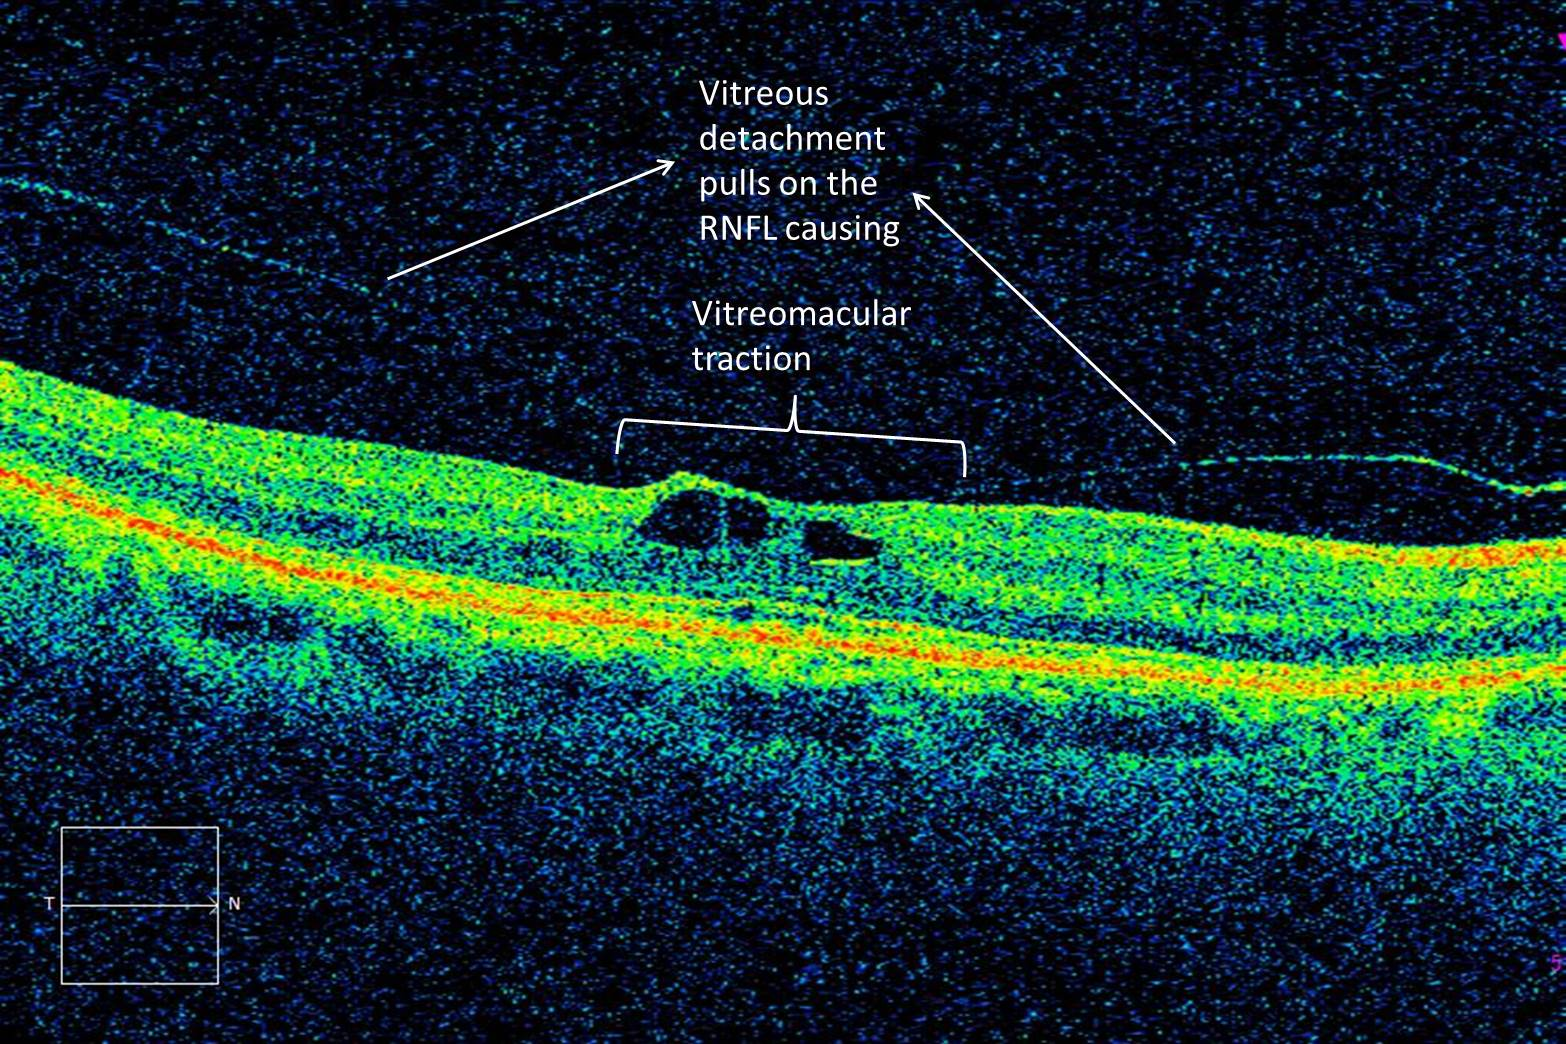
\includegraphics[width=0.3\textwidth, height = 0.15\textheight]{./content/method/figures/Vitreomacular}}\
   \subfigure[Rethinal thickening.]{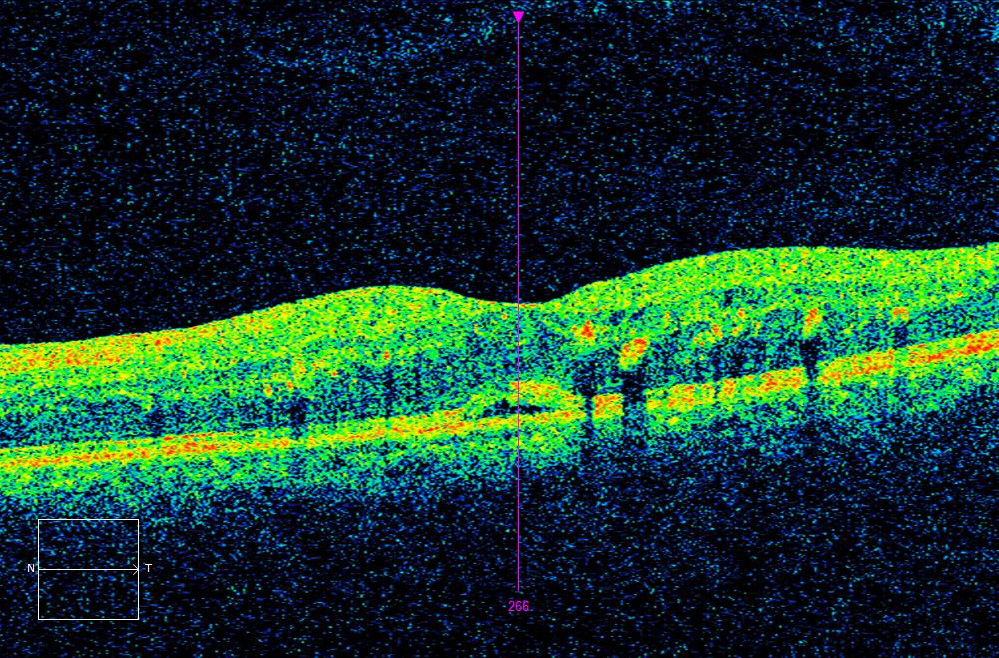
\includegraphics[width = 0.3\textwidth,height = 0.15\textheight]{./content/method/figures/RE}} \
   \subfigure[Cyst spaces, causing central and parafoveal retina thickening.]{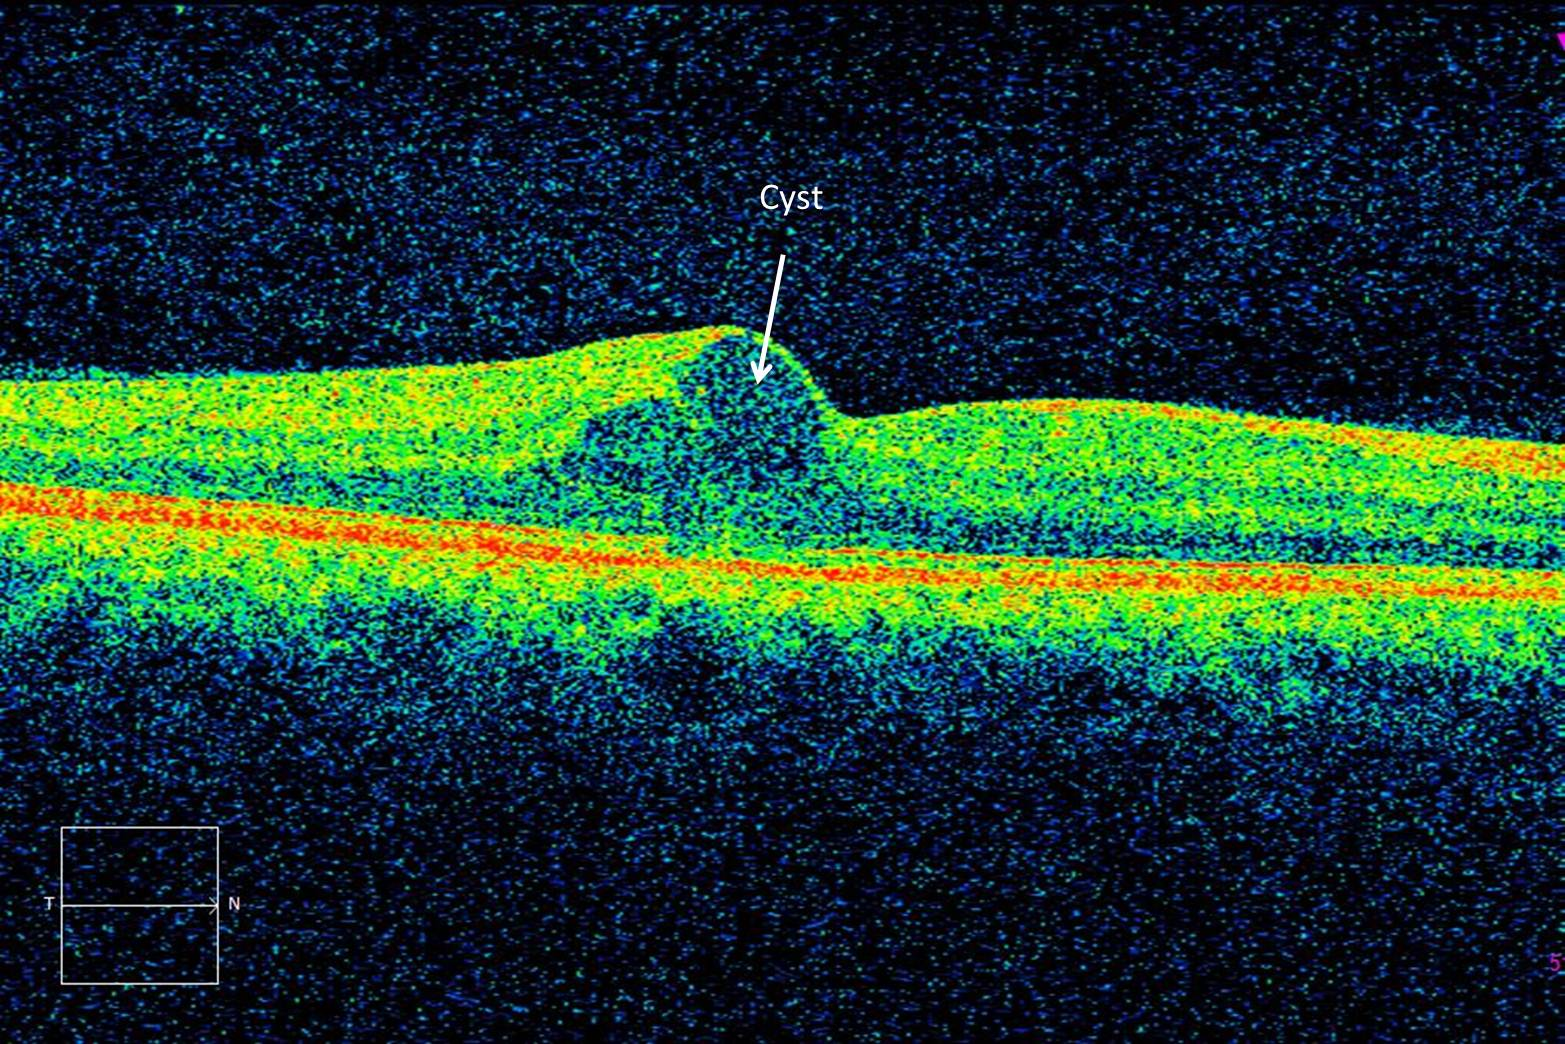
\includegraphics[width=0.3\textwidth,height = 0.15\textheight]{./content/method/figures/Cyst}}\\
   \subfigure[Cyst spaces and hard exudates, causing central retinal thickening.]{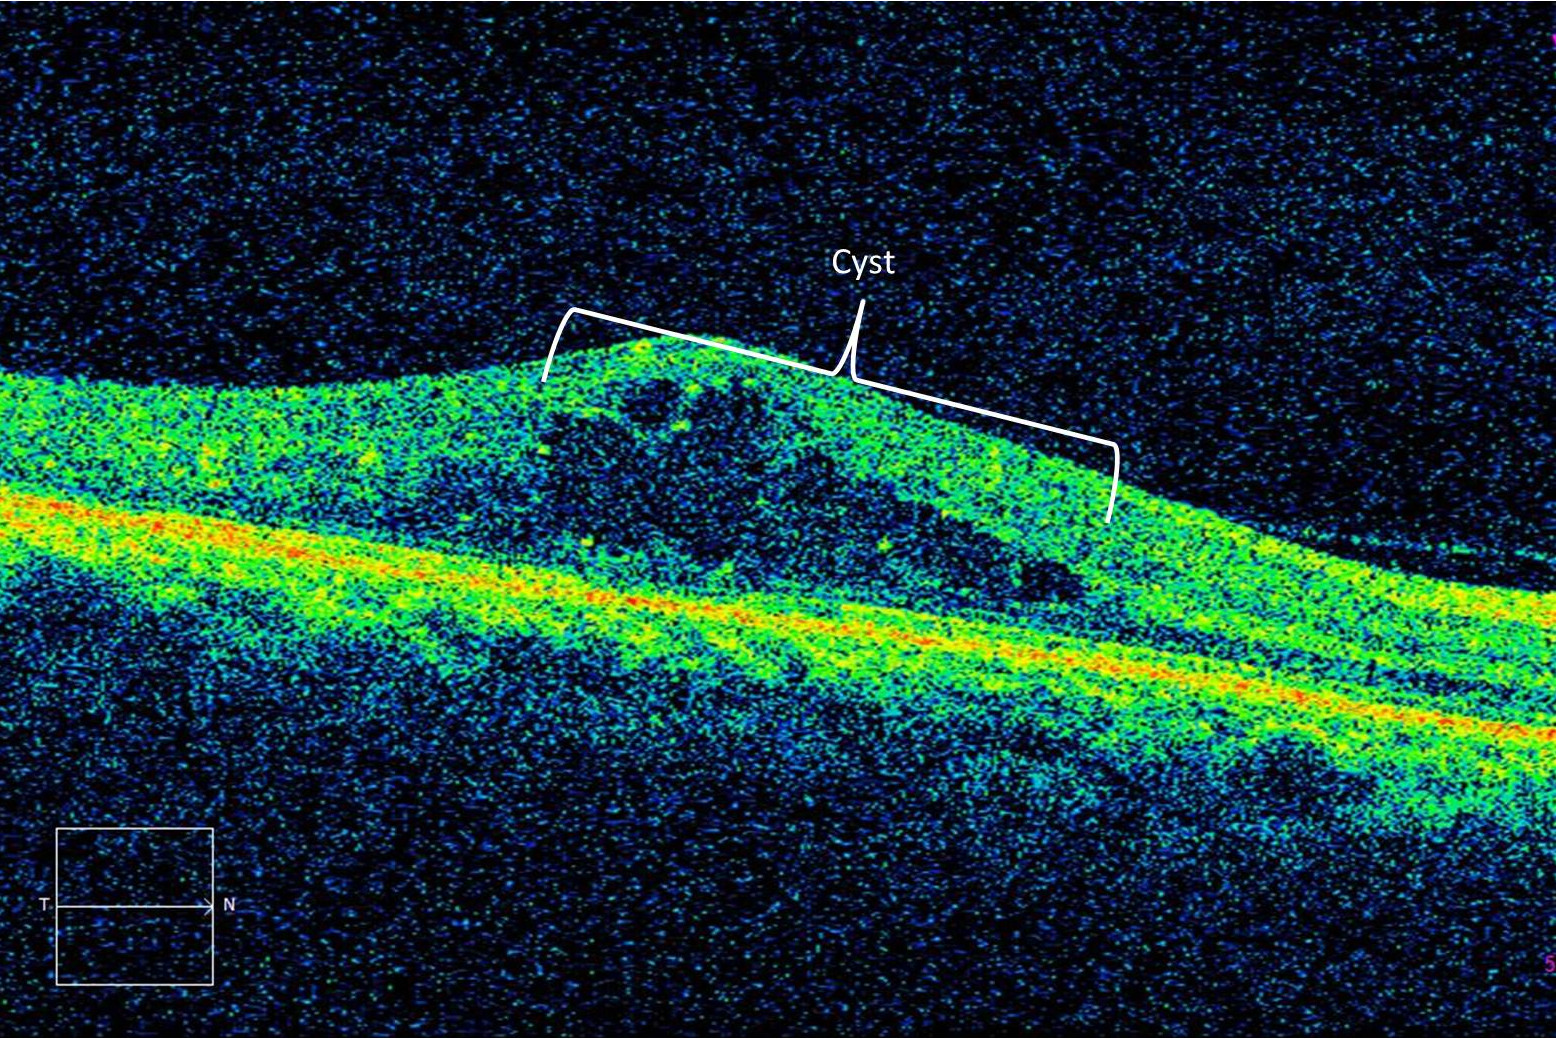
\includegraphics[width = 0.3\textwidth,height = 0.15\textheight]{./content/method/figures/Cyst+HE+RE}} \
   \subfigure[CSR (subretinal fluid), causing central and parafoveal thickening.]{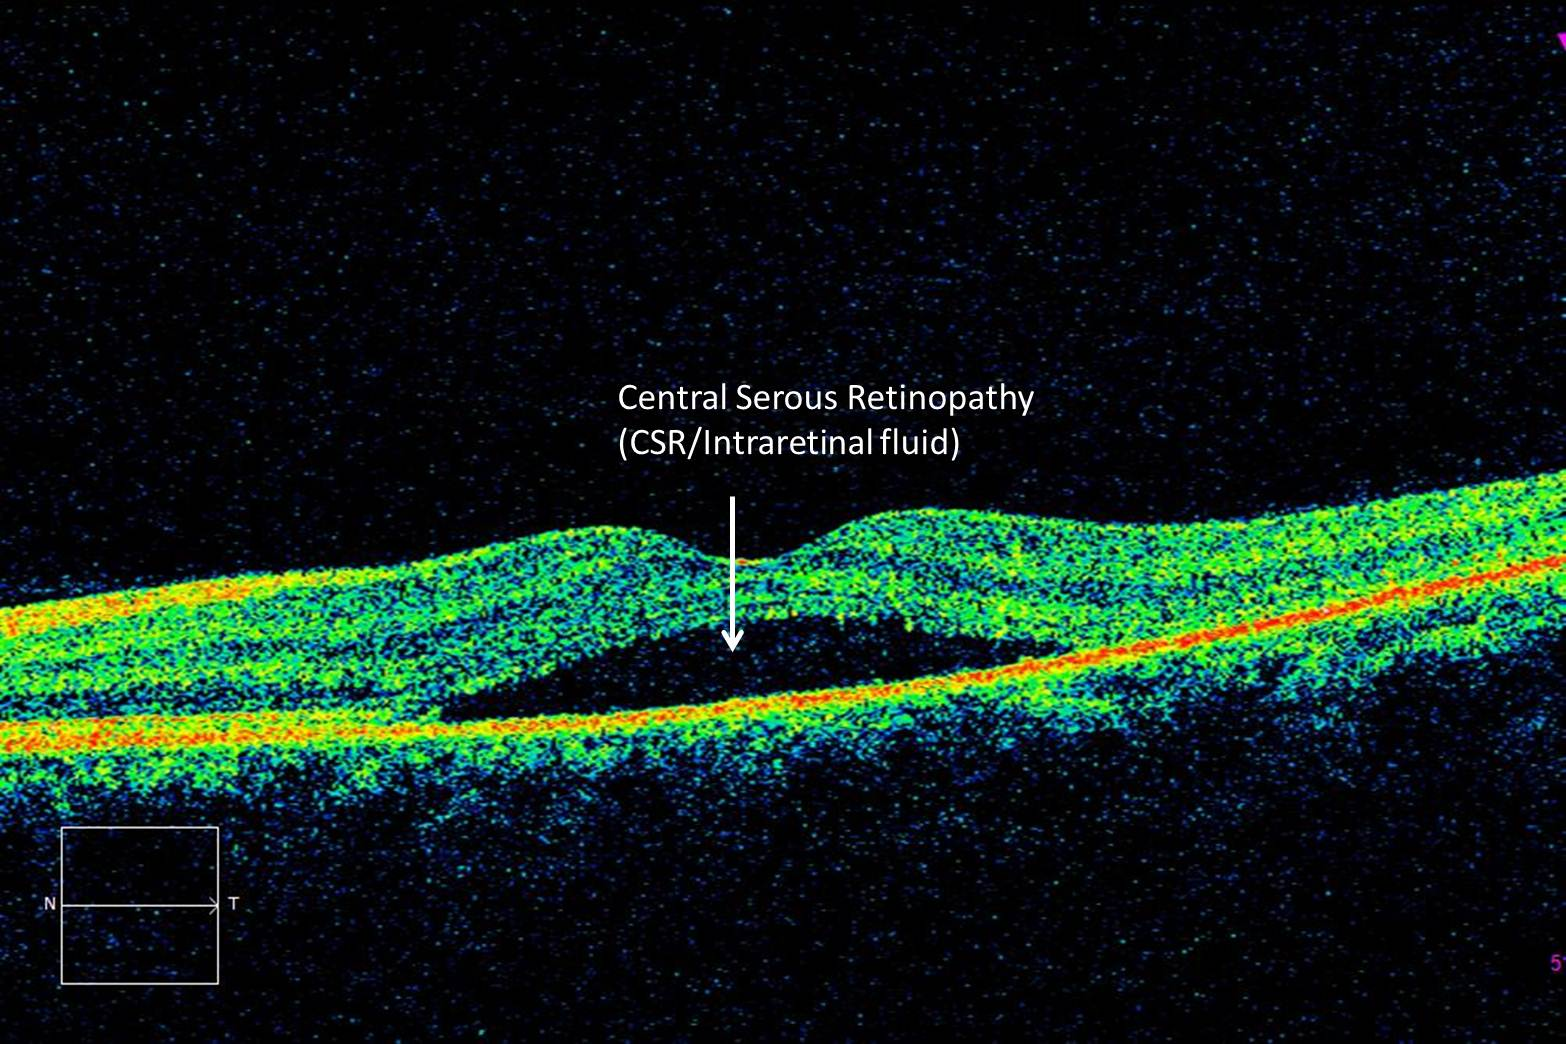
\includegraphics[width = 0.3\textwidth,height = 0.15\textheight]{./content/method/figures/CSR}} \
   \subfigure[CSR, hard exudates and cyst spaces.]{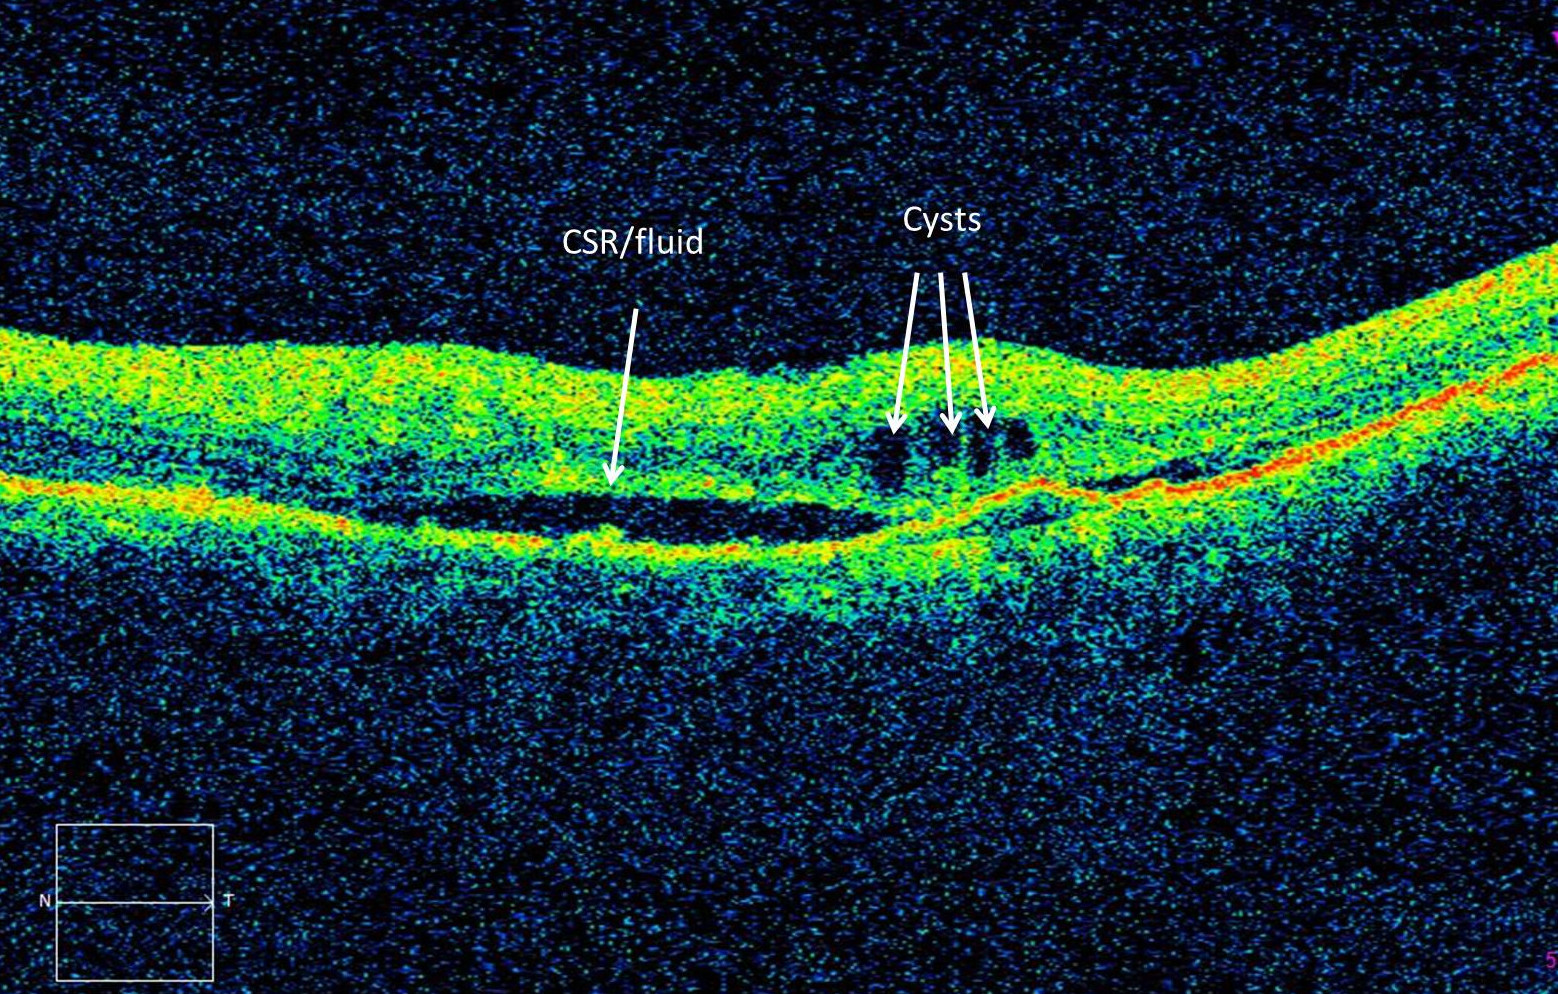
\includegraphics[width = 0.3\textwidth,height = 0.15\textheight]{./content/method/figures/Cyst+CSR+HE}} \\
   \subfigure[Cyst spaces, causing retinal thickening.]{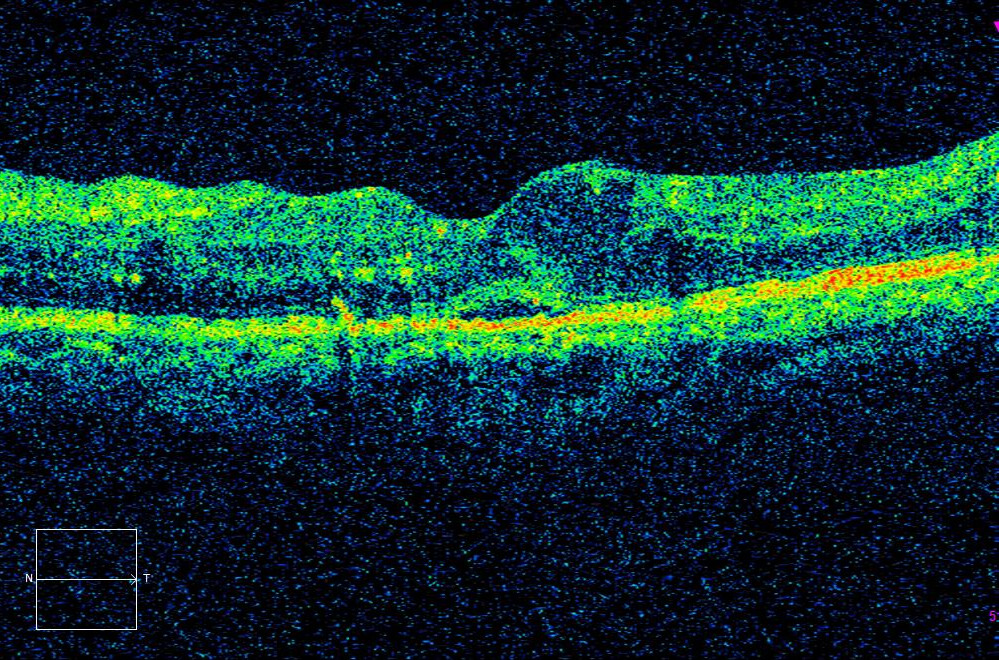
\includegraphics[width = 0.3\textwidth,height = 0.15\textheight]{./content/method/figures/Cyst+RE}} \
   \subfigure[CSR and hard exudates, causing retinal thickening.]{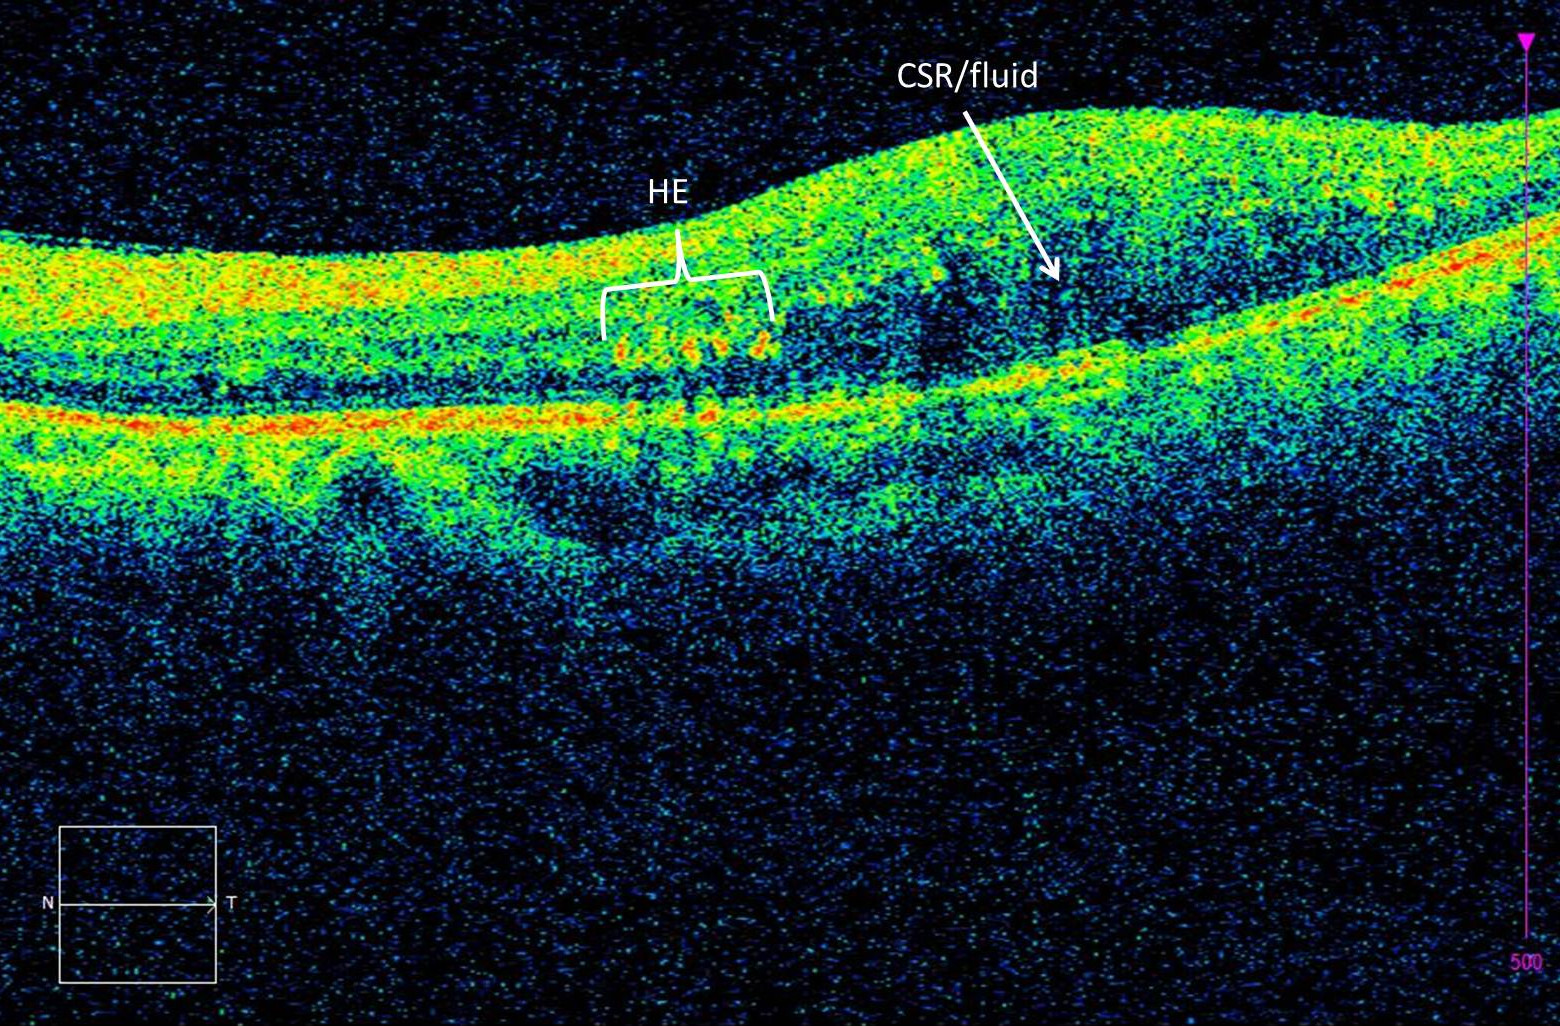
\includegraphics[width = 0.3\textwidth,height = 0.15\textheight]{./content/method/figures/CSR+HE+RE}} \   
   \subfigure[Cyst spaces causing parafoveal thickening.]{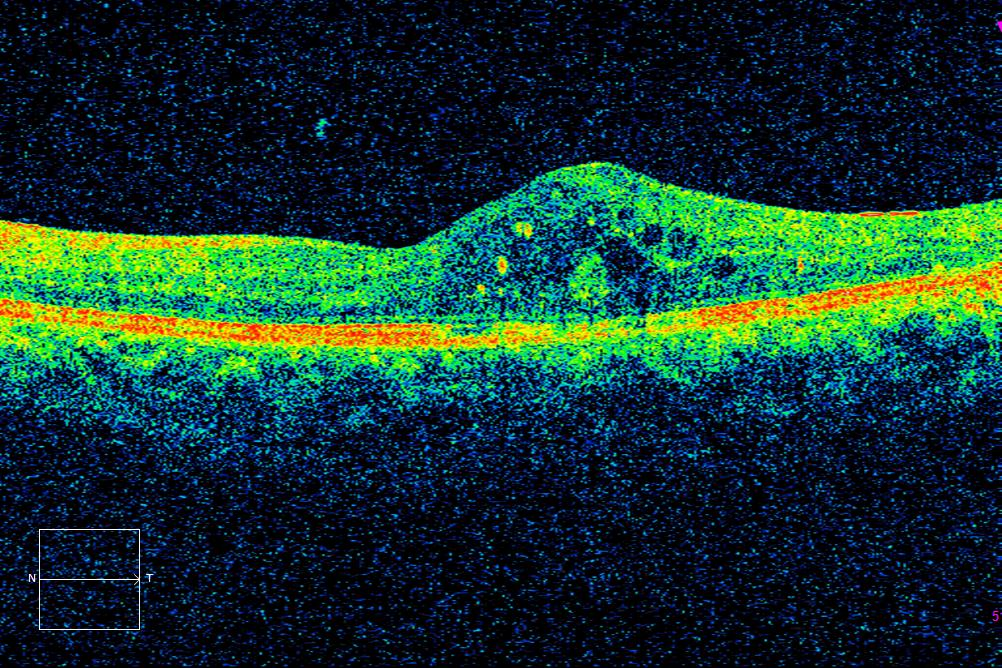
\includegraphics[width = 0.3\textwidth,height = 0.15\textheight]{./content/method/figures/Cyst+RE_parafovel}} \\
    
\end{center}
    \caption{Examples of \gls{dme} cases in \gls{seri} dataset.}
  \label{fig:bbdd}
\end{figure*}


\subsection{Semi-supervised methods}

Sankar~\textit{et~al.} propose to use a semi-supervised strategy to classify \gls{dme} \emph{vs.} normal \gls{oct} volumes based on appearance modeling of normal \gls{oct} images using \gls{gmm}~\cite{sankar2016classification}.
The main difference between this method and the supervised methodologies lies in the fact that only normal volumes are used to train the system.

For each \gls{oct} volume, the B-scans are denoised using \gls{nlm} filtering, flattened, and resized to ensure homogeneous dimension across all volumes.
Each B-scan is vectorized and projected into a lower-dimensional space with $p$ dimensions using \gls{pca}.
Subsequently, normal B-scans are modelled using a \gls{gmm} in which the number of mixture components $K$ is determined on a validation set.
At the testing stage, a scan is classified as normal or \gls{dme} depending of its Mahalanobis distance to the learnt model; if the distance is greater than the $97.5 \%$ quantile of the Chi-squared distribution with $p$ degree of freedom.
Therefore, a volume is classified as abnormal if the number of abnormal slice is greater than a given threshold, previously determined during the validation procedure.
A \gls{se} and \gls{sp} of $93.8 \%$ and $80.0 \%$ are respectively achieved on a cohort of 32 patients.

\begin{table*}
  \caption{Correspondence between the most relevant methodologies reviewed in Sect.\,\ref{sec:review} and the proposed experimental framework.}
% \resizebox{1\linewidth}{!}{
\centering
\footnotesize{
\begin{tabular}{l c	c c c c }
\toprule
\multicolumn{1}{c}{Ref} & Pre-processing & Features &  Mapping &  Representation & Classification\\
    &  &  &  &  & \\
\midrule
	&  &  &  &  & \\
%Venhuizen~\textit{et~al.}~
\multirow{2}{*}{Venhuizen~\textit{et~al.}~\cite{Venhuizen2015,venhuizen2015feb-repoICPR}} &  & \multirow{2}{*}{Texton} & \multirow{2}{*}{Local}   &\gls{pca} & \multirow{2}{*}{\gls{rf}} \\
	&  &  &  & \gls{bow} & \\
	&  &  &  &  & \\
%Srinivansan~\textit{et~ al.}
\multirow{3}{*}{Srinivasan~\textit{et~al.}~\cite{Srinivasan2014, srinivasan2014oct-repoICPR}} & Denoising (\gls{bm3d}) & \multirow{3}{*}{\gls{hog}} & \multirow{3}{*}{Global} & &  Linear- \\
 & Flattening & & & &\gls{svm} \\
 & Cropping & & & & \\
	&  &  &  &  & \\
%Lema\^itre~\textit{et~al.}~
\multirow{3}{*}{Lema\^itre~\textit{et~al.}~\cite{Lemaintre2015miccaiOCT, lemaitre2015apr-repoICPR}} & \multirow{3}{*}{ Denoising (\gls{nlm}) } & \gls{lbp} & Local &  \gls{pca} &  \multirow{3}{*}{\gls{rf}} \\
& & \gls{lbptop} & Global & \gls{bow}& \\
	&  &  &  &Histogram & \\
&  &  &  &  & \\

\multirow{3}{*}{Alsaih~\textit{et~al.}~\cite{Alsaih2016apr-repoICPR}} & Denoising (\gls{bm3d}) & \gls{lbp} & \multirow{3}{*}{Local} &  \gls{pca} &  Linear- \\
& Flattening & \gls{hog} &  & Histogram  & \gls{svm}\\
& Cropping & & & & \\
&  &  &  &  & \\

\multirow{2}{*}{Liu~\textit{et~al.}~\cite{Liu2011,liu20016apr-repoICPR}} & Flatten & Edge & \multirow{2}{*}{Local} & \gls{pca}& \gls{rbf}- \\
 & Aligned & \gls{lbp} & &\gls{bow} & \gls{svm} \\
 	&  &  &  &  & \\

%\midrule
\hdashline \noalign{\vskip 3pt}
\multirow{3}{*}{Sankar~\textit{et~al.}~\cite{sankar2016classification, sankar2015feb-repoICPR}} & Denoising (\gls{nlm}) & Pixel & \multirow{3}{*}{Global} & \multirow{3}{*	}{\gls{pca}} & Mahalanobis \\
 & Flattening &intensities & & & -distance\\
 & Cropping & & & & to \gls{gmm}\\
\bottomrule
\end{tabular}}
%}
\label{tab:survey-tab}
\end{table*}

%\begin{table*}
%\caption{Summary of the state-of-the-art methods.}
%\resizebox{1.05\linewidth}{!}{
%\scriptsize{
%\begin{tabular}{l ccc c cccc	c c c c	c c}
%\toprule
%Ref & \multicolumn{3}{c}{Diseases} & Data  & \multicolumn{4}{c}{Pre-processing} & Features & Representation & Classifier & Evaluation & Results\\
%    &  &  &  & size &  &  &  &  &  &  &  & & &\\
%   \cmidrule(l){2-4}\cmidrule(l){6-9}
%    & \gls{amd} & \gls{dme} & Normal  &           & De-noise & Flatten & Aligning & Cropping &   & &   &  &   \\
%\midrule
%& & & & & & & & & & & & & &  \\
%%Srinivansan\,\textit{et al.}~
%\cite{Srinivasan2014} & $\checkmark$ & $\checkmark$ & $\checkmark$ &  45 & $\checkmark$ & $\checkmark$ &  & $\checkmark$ & \gls{hog} &  & linear-\gls{svm} & \gls{acc} & 86.7\%,100\%,100\%  \\
%& & & & & & & & & & & & &    \\
%%Venhuizen\,\textit{et al.}~
%\cite{Venhuizen2015} & $\checkmark$ &  & $\checkmark$ & 384 &  & & & &  Texton  &\gls{bow}, \gls{pca}  & \gls{rf} & \gls{auc} & 0.984 \\
%& & & & & & & & & & & & &   & \\
%%Liu\,\textit{et al.}~
%\cite{Liu2011} & $\checkmark$ & $\checkmark$ & $\checkmark$  & 326 &  & $\checkmark$ & $\checkmark$ &  &  Edge, \gls{lbp} & \gls{pca}& \gls{svm}-\gls{rbf} &\gls{auc} & 0.93 \\
%& & & & & & & & & & & & & \\
%%Lema\^itre\,\textit{et al.}~
%\cite{Lemaintre2015miccaiOCT} &  & $\checkmark$ & $\checkmark$ & 62  & $\checkmark$ &  &  &  & \gls{lbp}-\gls{lbptop} & \gls{pca}, \gls{bow}, histogram&  \gls{rf} & \gls{se},\gls{sp} & 87.5\%, 75\%  \\
%& & & & & & & & & & & & &  \\
%\bottomrule
%\end{tabular}}}
%\label{tab:survey-tab}
%\end{table*}
[t]